\textbf{COLUNI 2020 -- Questão 31}\par\medskip Leia o texto.

\par

“O ‘Livre’ é um aplicativo de mobilidade urbana. A ferramenta é prática de utilizar e acompanha os avanços tecnológicos no setor de transporte. Com um celular nas mãos, de forma rápida, o cliente conecta com algum veículo disponível e, dentro de poucos minutos, é possível percorrer o trajeto desejado.” Disponível em: https://www.facebook.com/somoslivreapp/posts/794783470902864. Acesso em: 18 set. 2019.

\par

\textbf{Como funciona}

% COLUNI-AUTO-FIGURES-BEGIN
\begin{figure}[htbp]
\centering
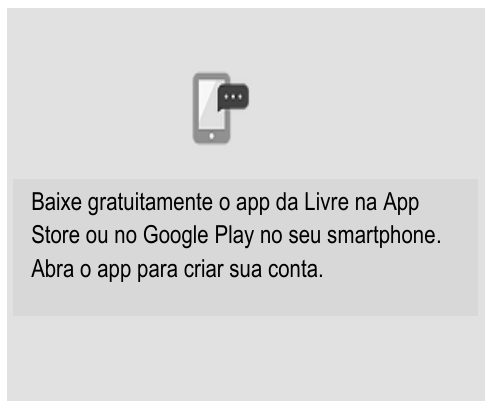
\includegraphics[width=0.95\linewidth]{static/simulados/coluni/figuras/2020/questao-31/figura-1.png}
\end{figure}
% COLUNI-AUTO-FIGURES-END

Baixe gratuitamente o app da Livre na App Store ou no Google Play no seu smartphone. Abra o app para criar sua conta.

% COLUNI-AUTO-FIGURES-BEGIN
\begin{figure}[htbp]
\centering
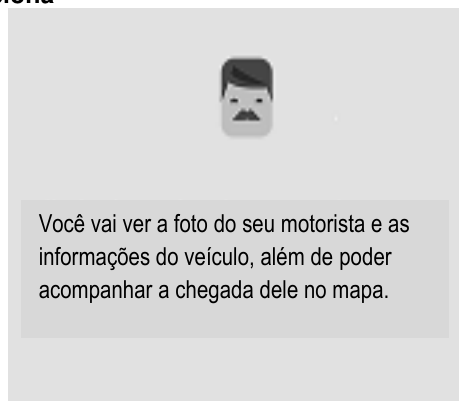
\includegraphics[width=0.95\linewidth]{static/simulados/coluni/figuras/2020/questao-31/figura-2.png}
\end{figure}
% COLUNI-AUTO-FIGURES-END

Você vai ver a foto do seu motorista e as informações do veículo, além de poder acompanhar a chegada dele no mapa.

% COLUNI-AUTO-FIGURES-BEGIN
\begin{figure}[htbp]
\centering
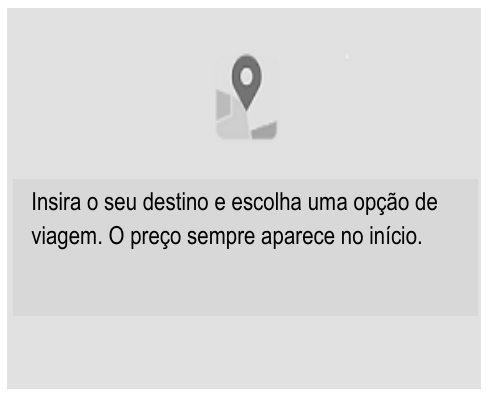
\includegraphics[width=0.95\linewidth]{static/simulados/coluni/figuras/2020/questao-31/figura-3.png}
\end{figure}
% COLUNI-AUTO-FIGURES-END

Insira o seu destino e escolha uma opção de viagem. O preço sempre aparece no início.

% COLUNI-AUTO-FIGURES-BEGIN
\begin{figure}[htbp]
\centering
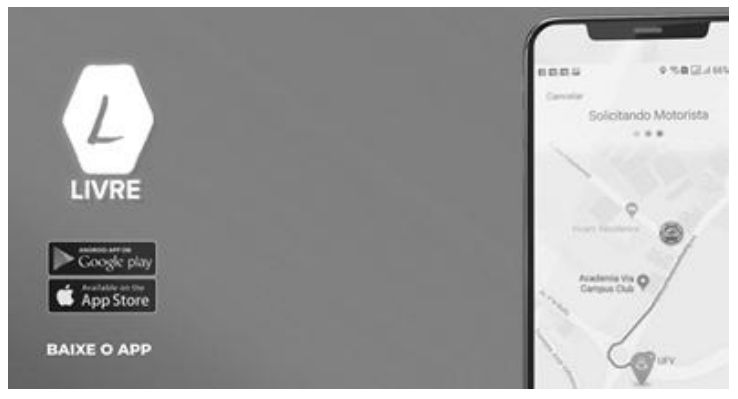
\includegraphics[width=0.95\linewidth]{static/simulados/coluni/figuras/2020/questao-31/figura-4.png}
\end{figure}
% COLUNI-AUTO-FIGURES-END

Disponível em: https://www.somoslivre.com. Acesso em: 18 set. 2019.

Sobre o referido aplicativo, assinale a afirmativa CORRETA:
\begin{enumerate}
\item Utiliza informações fornecidas pelo cadastro municipal de imóveis.
\item A visualização do trajeto é controlada apenas pelo motorista.
\item Utiliza instrumentos da cartografia.
\item Está disponível em todos os lugares e possibilita o acesso ao transporte público.\end{enumerate}
